\documentclass[11pt]{book}
 \usepackage[refpage]{nomencl} 
 \renewcommand{\nomname}{\sf\bfseries Glossary}
\usepackage{graphicx}
\usepackage{boxedminipage}
\usepackage{rhulcase}
\usepackage{upquote}
\usepackage{wrapfig}
\usepackage{upquote}
%\usepackage{boxedminipage}
\usepackage{hyperref}
\usepackage{amssymb}
\usepackage{amsmath}
\usepackage{listings}
\usepackage[dvipsnames]{xcolor}
\definecolor{codeColour}{rgb}{0.8,0,0}

\newcommand{\artVariable}[1]{\mbox{\color{purple}\em #1\/}}
\newcommand{\artConstructor}[1]{\mbox{\sf #1}}
\newcommand{\artCaseSensitiveLiteral}[1]{\mbox{\color{blue}\tt #1}}
\newcommand{\artCaseInsensitiveLiteral}[1]{\mbox{\tt #1}}
\newcommand{\artCharacterLiteral}[1]{\mbox{\tt #1}}
\newcommand{\artSpecial}[1]{\mbox{\color{orange}\sf\em #1}}
\newcommand{\artCatenation}{\ \ }
\newcommand{\artType}[1]{: #1}

\newcommand{\spacer}{\vspace*{1ex}\hrule\vspace*{1ex}}
\newcommand{\giftUnder}{\char`\^}
\newcommand{\giftOver}{\giftUnder\giftUnder}
\newcommand{\giftTear}{\giftUnder\giftUnder\giftUnder}
\newcommand{\ajstrut}{\rule[-0.2ex]{0pt}{1.9ex}}
\newcommand{\outdent}{\noindent\hspace*{-1.5cm}}
\newcommand{\outtext}[1]{{\outdent\normalsize\bf #1}}
\newcommand{\Con}{\color{black}$\blacksquare$}
\newcommand{\Coff}{\color{black}$\square$}
\newcommand{\todo}[1]{{\bf\color{red}** Todo: #1}}
\newcommand{\opboxdata}[1]{\rule[-2ex]{0pt}{5.5ex}\fbox{\parbox{2cm}{\begin{center}#1\end{center}}}}
\newcommand{\opbox}{\rule[-2ex]{0pt}{5.5ex}\fbox{\parbox{2cm}{\rule[-1ex]{0pt}{3.5ex}}}}

\newenvironment{CGL}{
\renewcommand{\arraystretch}{0.5}
\begin{tabular}{
 @{\hspace{0.5pt}}c@{\hspace{0.5pt}}c@{\hspace{0.5pt}}c@{\hspace{0.5pt}}c@{\hspace{0.5pt}}c@{\hspace{0.5pt}}c@{\hspace{0.5pt}}c@{\hspace{0.5pt}}c@{\hspace{0.5pt}}c@{\hspace{0.5pt}}c@{\hspace{0.5pt}}c@{\hspace{0.5pt}}c@{\hspace{0.5pt}}c@{\hspace{0.5pt}}c@{\hspace{0.5pt}}c@{\hspace{0.5pt}}c@{\hspace{0.5pt}}}
}
{
\end{tabular}
}
\newcommand{\pget}[1]{\par\vspace{1ex}\begin{center}\includegraphics[width=10cm]{#1}\end{center}\par\vspace{1ex}}

\lstnewenvironment{codeblock}{\lstset{language=Java,
columns=fullflexible, 
basewidth=0.51em,
basicstyle=\color{codeColour}\sffamily,
showstringspaces=false,
numbers=left, numberstyle=\tiny, stepnumber=1, numbersep=5pt,
xleftmargin=-0.2cm,
xrightmargin=-0.3cm,
frame=tl,
escapeinside={AJLOPEN}{AJLCLOSE}
}
\vspace{2ex}
}{\vspace{2ex}}

\lstnewenvironment{outputblock}{\lstset{
columns=fullflexible, 
basewidth=0.51em,
basicstyle=\color{black}\ttfamily,
showstringspaces=false,
xleftmargin=-0.2cm,
xrightmargin=-0.3cm,
frame=tl,
escapechar=£
}
\vspace{2ex}
}{\vspace{2ex}}

\lstnewenvironment{povcodeblock}{\lstset{language=POV,
columns=fullflexible, 
basewidth=0.51em,
basicstyle=\color{codeColour}\sffamily,
showstringspaces=false,
xleftmargin=-0.2cm,
xrightmargin=-0.3cm,
frame=tl,
escapechar=£
}
\vspace{2ex}
}{\vspace{2ex}}

\lstnewenvironment{bnfblock}{\lstset{language=Java,
columns=fullflexible, 
basewidth=0.51em,
basicstyle=\color{codeColour}\sffamily,
showstringspaces=false,
xleftmargin=-0.2cm,
xrightmargin=-0.3cm,
frame=tl,
escapechar=£
}
\vspace{2ex}
}{\vspace{2ex}}

\newcommand{\portrait}[3]{
\frame{
\begin{columns}
 \begin{column}[c]{5cm}
\fbox{\includegraphics[width=4.5cm]{#1}}
\end{column}
\begin{column}{10cm}
#2\\
{\small\color{darkred}\url{#3}}
\end{column}
\end{columns}
}
}
% Abbreviated frame command
\newcommand{\ajframe}[2]{\begin{frame}\frametitle{#1}#2\end{frame}}
% Fragile frame
%\begin{frame}[fragile]
\newcommand{\ajfframe}[2]{\begin{frame}[fragile]\frametitle{#1}#2\end{frame}}
\newcommand{\bframe}{\begin{frame}~\end{frame}}

\makenomenclature
\newcommand{\gloss}[2]{{\em #1}\marginpar{\fbox{\tiny\em #1}}\nomenclature{#1}{#2}}
\newenvironment{codebox}{\par\noindent\scriptsize\begin{boxedminipage}[t]{\textwidth}\vspace*{1ex}\par}{\end{boxedminipage}\par\vspace*{1ex}\par\noindent}

\title{Software Language Engineering notes}
\author{Adrian Johnstone\\{\small\tt a.johnstone@rhul.ac.uk}}
\pagenumbering{roman}
\parskip 2ex
\parindent0pt
\begin{document}
\makecstitle
\pagenumbering{roman}
\setcounter{page}{1}
\tableofcontents
\setcounter{chapter}{-1} 
\chapter{The Royal Holloway course}
This chapter is for students studying Software Language Engineering at Royal Holloway where we approach the material in a particular order designed to allow students to complete their projects within the footprint of a one semester course. 

Holloway students start with internal syntax and reduction semantics and only then learn about external syntax parsers and the use of GIFT operators to generate terms in their chosen internal syntax, before moving on to attribute-action systems. After studying that core material we look at topics in lexicalisation and ambiguity management. 

Experienced readers will note that this is a `semantics-first' approach: we encourage students to first enumerate the features of their language as a set of signatures, then write reduction rules to interpret those signatures, and only then to consider the external appearance of phrases in their language.

\begin{quote}
{\bf For readers who are not following the Holloway course:}\\[0.5ex] if you are using ART just as a parser, or have a particular interest in one or other approach to semantics you may want to take a different route and should probably skip straight to Chapter 1.
\end{quote}
\clearpage
\section{Aims and motivation}
Welcome to the Software Language Engineering course. You have been engineering {\em with} software languages for at least two years now. This course, though, is about the
engineering {\em of} software languages: you will learn how to build languages using concise formal notations
from which the implementation could be automatically generated.

All forms of engineering are a mixture of creative insight and disciplined implementation. For instance, the
architect of a bridge relies on structural engineers who can take a high level design and perform detailed
calculations on that structure to test whether it will withstand daily use. Ideally, this would be true for software too: our creativity would be expressed only through sound and
principled techniques; that is techniques that have been found to be safe and efficient using mathematical
and other forms of analysis.

In practice we mostly write software in a hopeful way, and then use testing to try and fill the gaps in
our understanding. Unfortunately, programming languages are inherently difficult to test since they are
designed to be flexible notations with very many combinations of interacting features.

We aim to tame this complexity by using {\em high level abstractions} that allow us to see the
specification of a complete language in a few pages. We can then use this specification to guide either a
hand crafted, efficient implementation, or automatically generate interpreters for the language which will
probably be less efficient, but may be adequate for many applications.

The overall goal is to make language processors that can be comfortably maintained and extended by the
engineers that take forward our work after we have moved on to other projects. To do that, we need to
provide concise, self documenting descriptions of the syntax and semantics of our languages that everybody
can understand and work with.

\section{Learning outcomes}
After working through these notes, you will
\begin{quotation}
\parskip1ex
\noindent 1. know how to use {\em Context Free Grammar} rules to define programming language syntax;

\noindent 2. be able to use grammar idioms and the {\em GIFT annotations} to create {\em derivation trees} with useful properties;

\noindent 3. understand how to write {\em reduction semantics} rules that the eSOS interpreter uses to execute programs;

\noindent 4. be able to write {\em attribute-action rules} that the attribute evaluator uses to execute programs;

\noindent 5. understand the types and operations of a {\em Value system}, and how to use a {\em plugin} to connect to Java classes; and

\noindent 6. be able to recognise ambiguity in language specifications and progressively eliminate it using {\em choosers}.
 \end{quotation}
\section{Assessment}
Your command of these learning outcomes will be assessed {\em via} a substantial personal project and an invigilated examination, each component being worth 50\% of the final mark. 

The project work is to be submitted at the end of the course, and requires the following four deliverables.
\begin{enumerate}
\item {\tt reduction.art} - a reduction semantics interpreter specified by eSOS rules and a context free grammar annotated with GIFT operators.
\item {\tt attribute.art} - an attribute-action interpreter specified by a context free grammar annotated with attributes and actions written as Value expressions.
\item {\tt ARTPlugin.java} - a plugin which connects your interpeters to your chosen domain specific actions
\item {\tt report.pdf} - a concise report highlighting interesting and novel features, along with example programs that work with both interpreters.
\end{enumerate}

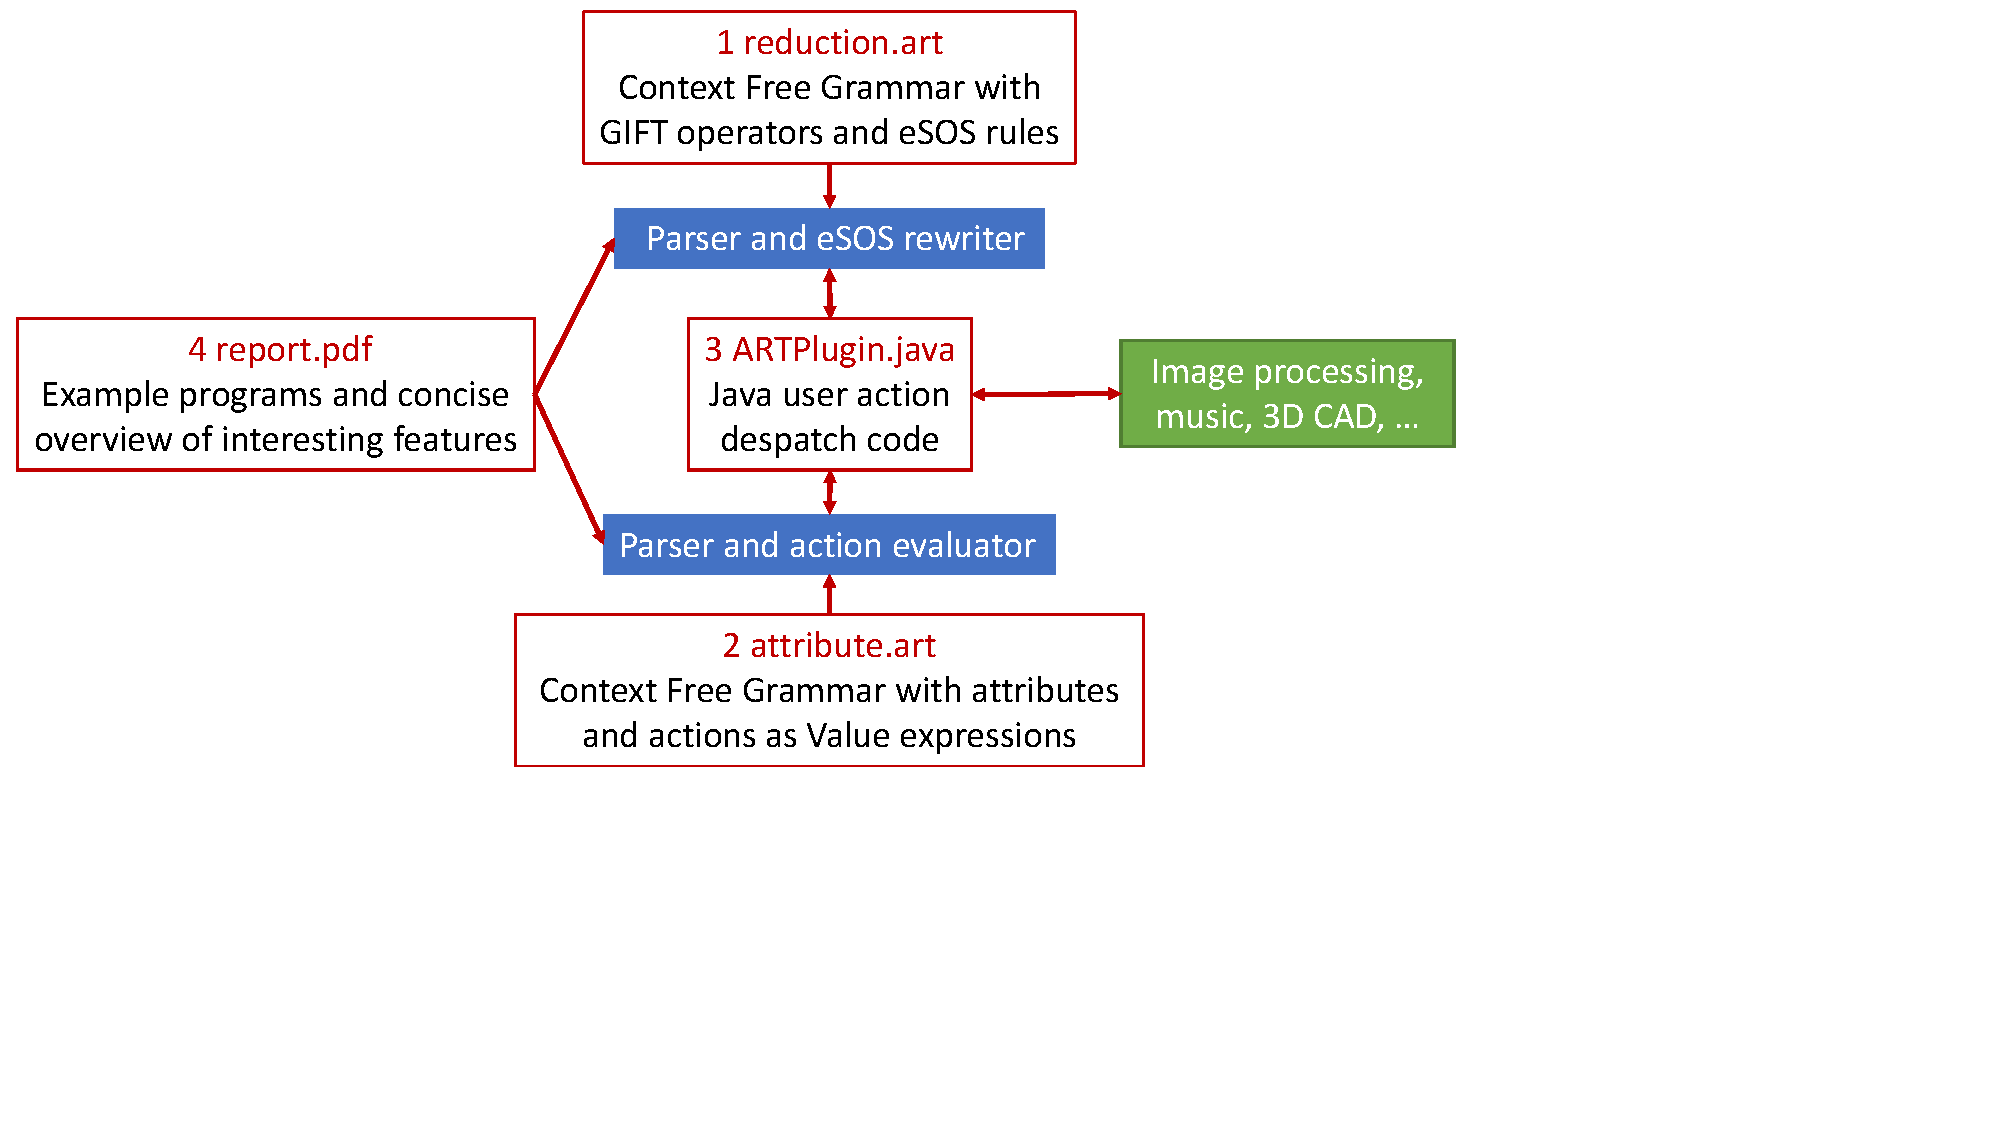
\includegraphics[scale=0.5,trim={0.25cm 5.8cm 9cm 0},clip]{project.pdf}

The blue boxes above represent language execution mechanisms that are built into the ART tool; their behaviour is specified by the rules that you write in {\tt reduction.art} and {\tt attribute.art}. The green box represents arbitrary Java code that you can connect to {\em via} a despatch routine in {\tt ARTPlugin.java}. You demonstrate the utility of your language using example programs listed in {\tt report.pdf}

After each weekly lab session, you will submit a snapshot of your work. These snapshots will not be assessed, but will be automatically analysed so that your progress can be tracked. If you are falling behind then you {\em must} ask for help.
\section{Project topics}
The focus of this course is on the constructs of general purpose programming languages, but to motivate the project work we offer three project variants to construct a {\em Domain Specific Language} for 
\begin{enumerate}
\item music generation {\em via} the Java MIDI interface;
\item image processing using the two-dimensional (2D) features of Java FX; and
\item Computer Aided Design for 3D printing using an extended form of the three-dimensional (3D) features of Java FX.
\end{enumerate}
You must commit to one of these topics by the end of the week 2 lab. To help you decide, please read the background material on each of these in Appendices~\ref{music:chapter}, \ref{ip:chapter} and \ref{3d:chapter}.


\section{Teaching week by week}
So as to help you prepare your project submission in a timely manner, we approach the learning outcomes in this order.
\begin{tabbing}
Week~~\=Chapter~~\=Lecture topic~~~~~~~~~~~~~~~~~~~~~~~~~~~~~\=Laboratory session\\[1ex]
1\>1\>Two interpreters for GCD\> Alero 3D design\\
2\>3\>Terms and pattern matching\> termTool \\
3\>4\>eSOS\> eSOS for expressions\\
4\>3\>The ART Value system\> eSOS for control flow\\
5\>2\>Context Free Grammars\> OSBRD parsing\\
6\>2\>GIFT operators\> Generation of eSOS terms\\
7\>5\>Attribute-action interpreters\>mini expression languages \\
8\>5\>Delayed attributes\> mini control flow languages\\
9\>2\>Paraterminals and lexicalisation\> mini with custom token patterns\\
10\>2\>Ambiguity management\> lexical and phrase level choice\\
\end{tabbing}

\chapter{First examples}
\setcounter{page}{0}
\pagenumbering{arabic}
\pagestyle{headings}
\noindent Here is an extract from the Pascal report\\[2ex]
\begin{boxedminipage}{\textwidth}
\sf\parindent0pt\parskip1ex
{\bfseries 9.2.2.1. If statements. }

The if statement specifies that the statement following the symbol then be executed only if the Boolean expression
yields true. 

IfStatement = ``if'' BooleanExpression ``then'' Statement
\end{boxedminipage}

\vspace*{2ex}

\noindent Here is a corresponding extract from one of the draft ANSI-C standards:\\[2ex]
\begin{boxedminipage}{\textwidth}
\sf\parindent0pt\parskip1ex
{\bfseries 6.8.4 Selection statements}

Syntax

{\em selection-statement:\\\hspace*{2em}
if ( expression ) statement
}

Semantics

A selection statement selects among a set of statements depending on the value of a
controlling expression.

A selection statement is a block whose scope is a strict subset of the scope of its
enclosing block. Each associated substatement is also a block whose scope is a strict
subset of the scope of the selection statement.

{\bfseries 6.8.4.1 The if statement}

Constraints

The controlling expression of an if statement shall have scalar type.

Semantics

The substatement is executed if the expression compares unequal to 0.
\end{boxedminipage}
\clearpage


\noindent And here is an extract from one of the {\em Java Language Specification} documents:\\[2ex]
\begin{boxedminipage}{\textwidth}
\sf\parindent0pt\parskip1ex
{\bfseries 14.9. The if Statement}

The if statement allows conditional execution of a statement.

{\em IfThenStatement:\\\hspace*{2em}
    if ( Expression ) Statement
}

\noindent The Expression must have type boolean or Boolean, or a compile-time error occurs.

{\bfseries 14.9.1. The if-then Statement}

An if-then statement is executed by first evaluating the Expression.

If evaluation of the Expression completes abruptly for some reason, the if-then statement completes abruptly for the same reason.

Otherwise, execution continues by making a choice based on the resulting value:
\begin{itemize}
\item If the value is true, then the contained Statement is executed; the if-then statement completes normally if and only if execution of the Statement completes normally.

\item If the value is false, no further action is taken and the if-then statement completes normally.
\end{itemize}
\end{boxedminipage}

All three extracts describe the same language feature: the simple conditional statement. If we write in C or Java the program fragment\begin{quote} \verb+z = 0; if (x == y) z = 3;+\end{quote}
then we expect that after execution the variable {\tt z} will hold the value 3 only if the variables {\tt x} and {\tt y} hold the same value. We get the same effect in Pascal by writing \begin{quote}\verb+z := 0; if x = y then z := 3;+\end{quote}
From these examples we can deduce the following:
\begin{itemize}
\item All three languages have conditional statements that `do the same thing' in some sense;
\item the textual form of the program fragments for Java and C are the same, but the Pascal fragment has a different form, even though the meanings are the same.
\end{itemize}
In programming languages, the meaning of a fragment is best thought of as its effect on the \gloss{state}{the set of values maintained by a program} of the computer, where the state is the set of values maintained by a program, which could simply be the contents of the computer's memory along with any changes to the computer's input and output devices.
\clearpage
We call the written form of a programming language fragment its \gloss{syntax}{the written form of a language}.

We call the meaning of a fragment its \gloss{semantics}{the meaning of a language} (that is the effect on the state of the computer).

\section{Specification styles for semantics}
The extracts above from Pascal, C and Java language standards are all trying to explain the syntax and semantics of a conditional statement. In each case the semantics is described in careful English prose (what we might call `legalistic' English) but with differing levels of detail. Nearly all programming language standards adopt this approach, but it is not ideal because it is hard to check that a prose specification is complete (that is, there aren't any special cases that have been left undefined) and consistent (that is, that there aren't any conflicting statements). It is even harder to check that a programming language processor, such as the Java compiler, correctly implements all aspects of the standard. Since so much of modern life is mediated by software written in programming languages, this vagueness in the underlying specification of languages and their implementations is worrying.

In an ideal world, we would have a commonly understood concise notation for describing the semantics of a language fragment with which we could construct arguments for the completeness and consistency of a programming language standard, and which we could use to check the correctness of compilers, interpreters and other language processors perhaps using a computer itself to do the checking. A semantics described this way would be called a \gloss{formal semantics}{}.

In fact such notations do exist, but they have not been widely adopted by programming language designers, for perhaps two reasons: firstly they are conventionally presented in a mathematical style that deters many software practitioners; and secondly complete language descriptions are very dense and can be quite long. Now, the second reason is not a very good one, because legalistic English prose descriptions of semantics are also very dense and long: the Java Language Specification for Java 22 runs to 876 pages.

The ART tool that we are using here to study software language engineering contains an interpreter for one style of formal semantics called \gloss{Structural Operational Semantics}{} (SOS). 

Our particular version is called \gloss{eSOS}{}  because it allows certain parts of a specification to be elided away, which saves writing. 
eSOS is designed to appeal to those with a background in procedural languages: in Chapter~\ref{eSOS:chapter} we give programs that show how eSOS rules are interpreted so that software engineers can reason about the way in which their specifications will be processed. 

Now, some aspects of our presentation would induce a sharp intake of breath from those who prefer a more declarative and mathematically rigorous approach to semantics, but we hope that eSOS will de-mystify SOS for programmers who are wary of mathematical treatments, and perhaps encourage the use of SOS as a design and prototyping medium for domain specific languages where sometimes the only available language definition is the code of an implementation.

ART also suports \gloss{attribute-action}{} systems: a style of semantics that is common in traditional parser generators such as the Bison tool which is distributed with  most Unix systems; Chapter~\ref{attribute:chapter} describes the approach in detail. These kinds of specifications can usually be executed more efficiently than for an eSOS interpretation, but in our experience attribute-action systems are more likely to be incomplete or inconsistent (i.e. buggy) than an eSOS specification. In Chapter~\ref{advice:chapter} we discuss our preferred approach, which is to prototype in eSOS, and then if necessary transform to an equivalent attribute-action system to improve performance.
 
\section{Specification styles for syntax}

Although formal semantics has not achieved much traction with language designers, there is almost complete agreement that syntax should be specified using a {\em Context Free Grammar} (CFG), and that is evident in the extracts above; they all give a context free grammar rule for the syntax, although the notation used for the rule varies slightly.

For Pascal we have
\begin{quote}
\sf IfStatement = ``if'' BooleanExpression ``then'' Statement
\end{quote}
The doubly-quoted symbols are Pascal keywords. The other symbols are placeholders for language fragments. For instance, a {\sf BooleanExpression} could simply be the constant {\tt true} or an expression like {\tt x = y}.

Clearly the placeholders could represent arbitrarily long pieces of program but when focussing on the syntax and semantics of the conditional statement, we don't want to have to specify their exact form. This is an example of \gloss{abstraction}{the hiding of unnecessary detail}, that is the hiding of unnecessary detail so that we can focus on the matter in hand.

The purpose of a CFG rule, then, is to give a template for one feature of the language: the rule tells is that a conditional statement starts with the keyword {\tt if} which must be followed by an expression over the booleans, then the keyword {\tt then} followed by an arbitrary statement. Somewhere else in the grammar we expect to see definitions for the placeholders {\sf BooleanExpression} and {\sf Statement}. A complete set of such rules with no missing definitions is called a Context Free Grammar. ART contains tools for processing and visualising grammars in various ways that we shall discuss in Chapter~\ref{cfg:chapter}.

\section{A complete example: GCD}

The algorithm we shall use is Euclid's integer Greatest Common	Divisor method, described in the second proposition of {\em Elements VII} some 2,300 years ago. It is worth looking up the original description which is written in quite verbose prose. 

Here is a version written in Java.
\begin{codeblock}
import java.util.Scanner;

public class GCD {
  public static void main(String[] args) {
    int a, b;
    Scanner input = new Scanner(System.in);

    a = input.nextInt();
    b = input.nextInt();

    input.close();

    while (a != b)
      if (a > b)
        a = a - b;
      else
        b = b - a;

    System.out.println(a);
  }
}\end{codeblock}
Java programs need quite a lot of setting up and anyway this is a course on language design, so let us construct our own, more compact programming notation to express the same program. 
\begin{codeblock}
a := input(); 
b := input();

while a != b 
   if a > b
     a := a - b; 
   else
     b := b - a; 

output(a);
\end{codeblock}
\label{GCDCava}
We shall call this notation the GCD language. Note that assignment to a variable is denoted by \verb+:=+, not by \verb+=+. As in C and Java statements are terminated with (not separated by) a \verb+;+ The phrase \verb+input()+ reads a 32-bit integer value from the standard input stream, and \verb+output(a)+ appends a textual representation of the value of \verb+a+ to the output sequence. The names of numeric types indicate their precision: {\tt } is equivalent to {\tt Integer} in Java. Variable names are not pre-declared.
 
\subsection{The fixed-code-and-program-counter interpretation}
When we are developing software, we write code, load it into a development environment such as Eclipse and then run it to see if its behaviour matches our expectations. Figure~\ref{eclipse:gcd} shows a screenshot of the Java CGD program being run under the debugger within Eclipse. 

\begin{figure}
\hspace*{-2.5cm}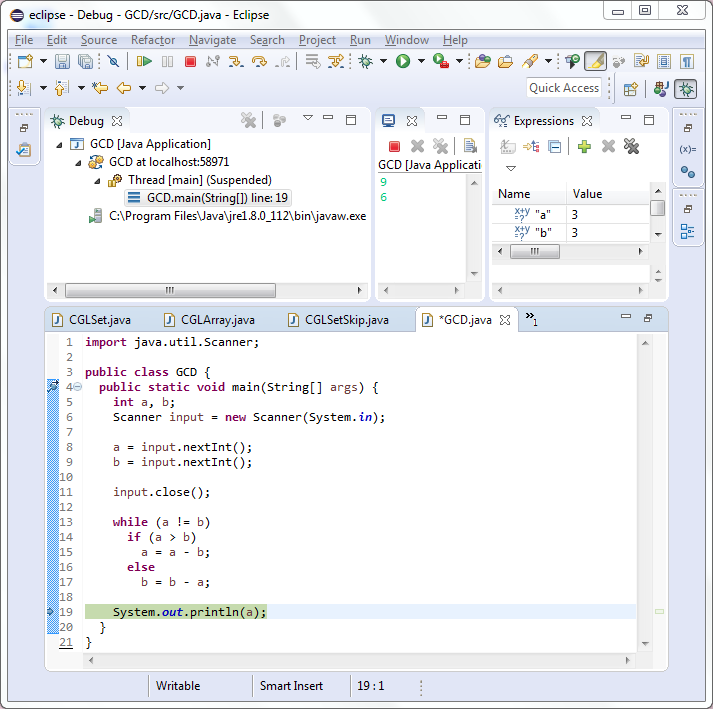
\includegraphics{png/GCDEclipse.png}
\vspace*{1cm}
\caption{Java GCD implementation during an Eclipse debug session}
\label{eclipse:gcd}
\end{figure}

We can see the program's Java code, the input $[ 9, 6 ]$ (in green) and the state of the store with variables {\tt a} and {\tt b}, both presently mapped to the value 3. The program has stopped just before executing the output statement. I can tell this because line 19 of the code window has a small pointer arrow on the left hand side and is highlighted in grey. In this system, I can execute one more line of code (moving the pointer to line 20) by pressing the `step-over' button.

This idea of code which is essentially fixed during a program's execution along with the use of a pointer (called the {\em program counter} or PC) is fundamental to most programmers' ideas of how computers operate. It is a direct legacy of the von Neumann architecture that is used in almost all modern computing devices: in these machines most programs are indeed static lists of instructions that reside in the store; and the instructions for a particular program do not change as it is being executed. The dynamic aspects of a program's execution are under the control of the PC which points to the next piece of code to be executed: at a branch point we may test a condition and update the PC with one of two values depending on that outcome. The sequence of values displayed by the program counter during a program's execution constitutes the {\em control flow} for this particular input. (We shall sometimes talk about the control flow of a {\em program} which is the union of the control flows exhibited by every possible input.)

This static-code-and-program-counter model breaks down for some situations. Firstly, since the instructions reside in the store, it is entirely possible for a running program to change its own instructions, and indeed some early processor architectures relied on this idea when executing subroutines. Such {\em self-modifying code} is widely recognised as being very difficult to reason about, and as a result almost no high level languages allow it. However, operating systems, and programming environments (such as Java) which allow dynamic loading of classes at run time do effectively present a form of self modifying code in a restricted way: we allow a completely new block of code to be loaded (possibly replacing an existing block or subprogram) and then pass control to it. During a load, the code is treated as passive data, and only once fully installed do we allow the PC to access its contents. We do not allow individual instructions within an executing piece of code to be changed. The hardware often enforces a policy in which the store is internally divided into 
{\em blocks} and at any one time a block is either read-only or writable. During a code load, the target blocks are made writable, but then changed to read-only when the code has been integrated. The PC is never allowed to hold an address from a writable block.

Now, although the hardware works with (mostly) static code and a program counter, that does not mean that a formal model of program execution must take the same view. Just as aviation pioneers had to learn that wing-flapping was not a useful way to get humans airborne (propellers and jet engines being a better engineering compromise) the pioneers of formal approaches to programming language semantics had to find a way of dispensing with the program counter. Why is this?

\subsection{What is equality?}
It turns out that the {\em substitution model of equality} that is used in most mathematical reasoning is much simpler than the {\em assignment model of equality} used in procedural programming languages. In mathematics, if I say $x = 3$ I mean that x and 3 are synonyms, and in fact anywhere that $x$ appears subsequently I could cross it out and write 3. In procedural programming languages like Java, if I write $x = 3$ I may subsequently write $ x= 4$, and so the relationship between $x$ and its value depends on the most recent assignment to $x$ under the history execution history  for a particular input. 

The substitution model is simple and easy to reason about; the assignment model is efficient in that identifiers (in detail, named cells with machine addresses) may be re-used rather than having to be maintained throughout the runtime of a program. There are languages that use substitution semantics: they are loosely called functional languages; Haskell is perhaps the purest of the functional languages. Other mostly-functional languages such as ML and Scheme do allow assignment, but the culture of programmers in those systems discourages assignment. In procedural languages, assignments are probably the most common operation performed during execution.

The use of assignment presents a challenge to formal analyses of program semantics, but it is particularly problematic that the program counter itself works by assignment. If we adhere strictly to von Neumann dogma, then we cannot even execute {\em functional} code without using assignment, and this is very uncomfortable.

\subsection{The reduction interpretation}
There is a straightforward way of thinking about program execution that does not require the use of a program counter. The trick is to think of the program code itself as something that can be progressively rewritten until all that we have left is a result. 

Consider this Cava program fragment
\begin{codeblock}
output(3);
output(10+2+4);
\end{codeblock}

The first thing the program does is output the value 3. We can represent this by constructing the output list $[3]$ and then discarding the first line of the program (since we do not need it again). There is a sense in which the tuple \begin{quote}$ $\verb^"output(3); output(10+2+4);"^, []$  $\end{quote} means the same thing as
\begin{quote}$ $\verb^"output(10+2+4);"^, [3]$  $\end{quote}
because the externally visible effect of starting with an empty output and executing lines 1 and 2 above is the same as starting with the output $[3]$ and only executing line 2. Let us therefore represent each step of a program's execution by a pair comprising the output and a program that represents only what remains to be done:
\begin{codeblock}
output(10+2+4); [3]
\end{codeblock}
Now we have to evaluate the expression 10+2+4 before we can execute the next output statement. In detail, the computer can only execute one arithmetic operator at a time; let us choose to execute 10+2, and rewrite it to the result 12.
\begin{codeblock}
output(12+4); [3]
\end{codeblock}
Now we do the other arithmetic operation: 12+4 is rewritten to 16.
\begin{codeblock}
output(16); [3]
\end{codeblock}
Finally we can execute the output statement, and add 16 onto the end of the output list.
\begin{codeblock}
[3, 16]
\end{codeblock}

Execution is now complete. Note that we could start in any of the five states above and end up with the same output.

We call this kind of display of machine states the {\em reduction semantics transition graph} for our program. Just as a sequence of CGL playing fields is a fragment of the graph of the transition relation for CGL, this trace is a fragment of the graph of the transition relation for Cava which is defined over tuples of $ $program, output$  $. It is a precise, architecture independent description of the step-by-step evaluation of our program. Do note, though, that we have not yet said anything at all about how that transition relation may be practically specified. In this example, and in the larger example in the next section, we have simply chosen plausible operations informally. Later on this book we shall use sets of {\em inference rules} to define the relation in a way which would allow the automatic generation of this style of reduction interpreter; and that will in fact be a true symbol-pushing formulation.
 
\subsection{A reduction evaluation of GCD with input [6, 9] }

A reduction semantics is so-called because we attempt to rewrite programs to values, which usually means replacing part of the program term with a smaller one, and thus reducing the program. Occasionally, though, we will actually rewrite terms to longer terms.

We now present the reduction semantics trace for the GCD program running on input $[6,9]$\,--\,exactly the program and input shown in the debugger screenshot in Figure~\ref{eclipse:gcd} . There are 36 steps in this trace, which make for intimidating reading, but bear in mind that a step (very roughly) corresponds to a machine operation such as fetching an operand or adding two numbers. Useful programs entail the execution of a {\em lot} of operations: some of the programs we run on modern processors take an appreciable amount of time to execute even though a 3GHz processor will, in two seconds, execute one instruction for every person on the planet\,---\,a number well beyond our abilities  to directly comprehend. This is just a roundabout way of saying that machine operations are fine grained, and we need an awful lot of them to do useful work. Any attempt to list all of the steps that are gone through by a non-trivial running program is going to generate a long list.

\lstMakeShortInline[language=Java,columns=fullflexible,basicstyle=\color{red}\sffamily]^

We shall use a slightly more compact form to display the steps. First, we shall write the entire program term on a single line: rather than the nicely laid out version shown on page~\pageref{GCDCava}, we say
\begin{quote}
\hspace*{-0.6cm}
^a:=input(); b:=input(); while a!=b if a>b a:=a-b; else b:=b-a; output(a);^
\end{quote}

In our initial example of a reduction trace, the complete state of the machine could be represented as a tuple containing a program term and an output list. All of the calculations used constants, so there was no need to represent the store, or any input. In the GCD program, we {\em shall} need these entities, so our trace will be a sequence of tuples $ I, S , P, T  $ displaying the current values for the input, store, output and term, respectively. The initial term has input $[6,9]$, an empty store and an empty output:

\begin{quote}
\hspace{-1.2cm}$  [6, 9], \{\ \}, [\ ],$ 
^a:=input(); b:=input(); while a!=b if a>b a:=a-b; else b:=b-a; output(a);^$  $
\end{quote}
\lstDeleteShortInline^

A physical store is a fixed set of cells, each with a fixed address but containing a value which may be changed. One mathematical model of a store is a map from identifiers to values, and we only put into the map those identifiers we need. Evaluating a {\em declaration} in the program term has the effect of creating a new store $S^\prime$ from $S$ which has all of the bindings in $S$ {\em and} the new binding required by the declaration. Assigning a new value to a variable has the effect of changing the mapping of one variable in the store, and using a variable in an expression requires us to look up the value mapped to the variable's identifier. We use the notation $X\mapsto y$ for an element of S, and the special symbol $\bot$ (read as `bottom') to represent the special value `none'. A declaration of $X$ with no associated initialisation of $X$ creates a binding $X\mapsto\bot$. In Cava, declarations are usually implicit, in that the first time we encounter an assignment to a variable $x$, we declare $x$ and perform the assignment together.

Each step of our trace involved identifying a part of the program term that we shall execute, and then rewriting the program term to represent what is left to do of the original term. We call the subterm that is to be replaced a {\em reducible expression} or {\em redex} for short. In the trace below, we have highlighted the chosen redex in red at each stage. Sometimes there is a choice of redexes available: for instance when processing the GCD program declarations for {\tt a} {\tt b}, it does not mater which order we process them in. We have chosen to do {\tt b} first.

A reduction semantics for linear code is straightforward, but we need to think carefully about loops. The approach we have taken here is to make use of a {\em program identity}, that is a program transformation that does not change the semantics of a program term, but does change the syntax, and thus the reduction trace. If we have a loop of the form

\begin{codeblock}
while booleanExpression do statement;
\end{codeblock}

then we can always transform it into

\begin{codeblock}
if booleanExpression { statement; while booleanExpression do statement; }
\end{codeblock}

We have effectively unpacked the first iteration of the loop and are handling it directly with an {\bf if} statement followed by a new copy of the {\tt while} loop which will compute any further iterations. When we have completed all of the iterations we shall encounter a term like

\begin{codeblock}
if false { statement; while booleanExpression do statement; }
\end{codeblock}
which rewrites to the empty subterm. This device, then, allows us to treat {\bf while} loops using only {\bf if} statements.

When reading the reduction trace below, the bold headings should simply be treated as comments: they are there to break up the reductions into related blocks as an aid to comprehension and have no part in the formal, symbol-pushing, description of program execution. At each step $i$, look for the highlighted redex: the tuple for step $i+1$ should contain a term which has all of the non-highlighted parts from step $i$, and some new (possibly empty) subterm which has replaced the redex. The entities will display any changes arising from side effects of the reduction, such as reading input, declaring a variable, redefining the value of a variable or writing to output.

\label{reduction:trace}
\lstMakeShortInline[language=Java,columns=fullflexible,basewidth=0.51em,basicstyle=\color{BlueViolet}\sffamily]|
\lstMakeShortInline[language=Java,columns=fullflexible,basewidth=0.51em,basicstyle=\color{BrickRed}\sffamily]@

{\small\parskip2ex
\outtext{Start of trace}

\outtext{Initialise variables from input}

\outdent$  [6, 9],\{\},[\ ],$ 
@a:=input(); @|b:=input(); while a!=b if a>b a:=a-b; else b:=b-a; output(a);|$  $

\outdent$  [9],\{a \mapsto 6\},[\ ],$ 
@b:=input(); @|while a!=b if a>b a:=a-b; else b:=b-a; output(a);|$  $

\outtext{Rewrite using {\tt while p s} $\rightarrow$ {\tt if p \{ s ; while p s \}}}

\outdent$  [\ ],\{a \mapsto 6, b \mapsto 9\},[\ ],$ 
@while a!=b if a>b a:=a-b; else b:=b-a;@| output(a);|$  $

\outtext{Evaluate $ a \ne b$ with store $\{a \mapsto 6, b \mapsto 9\}$}

\outdent$  [\ ],\{a \mapsto 6, b \mapsto 9\},[\ ],$ 
|if |@a@|!=b { if a>b a:=a-b; else b:=b-a; while a!=b if a>b a:=a-b; else b:=b-a; } output(a);|$  $

\outdent$  [\ ],\{a \mapsto 6, b \mapsto 9\},[\ ],$ 
|if 6!=|@b@| { if a>b a:=a-b; else b:=b-a; while a!=b if a>b a:=a-b; else b:=b-a; } output(a);|$  $

\outdent$  [\ ],\{a \mapsto 6, b \mapsto 9\},[\ ],$ 
|if |@6!=9@| { if a>b a:=a-b; else b:=b-a; while a!=b if a>b a:=a-b; else b:=b-a; } output(a);|$  $

\outdent$  [\ ],\{a \mapsto 6, b \mapsto 9\},[\ ],$ 
@if true { if a>b a:=a-b; else b:=b-a; while a!=b if a>b a:=a-b; else b:=b-a; }@| output(a);|$  $

\outtext{Evaluate $ a > b$ with store $\{a \mapsto 6, b \mapsto 9\}$}

\outdent$  [\ ],\{a \mapsto 6, b \mapsto 9\},[\ ],$ 
|if |@a@|>b a:=a-b; else b:=b-a; while a!=b if a>b a:=a-b; else b:=b-a; output(a);|$  $
 
\outdent$  [\ ],\{a \mapsto 6, b \mapsto 9\},[\ ],$ 
|if 6>|@b @| a:=a-b; else b:=b-a; while a!=b if a>b a:=a-b; else b:=b-a; output(a);|$  $
 
\outdent$  [\ ],\{a \mapsto 6, b \mapsto 9\},[\ ],$ 
|if |@6>9 @| a:=a-b; else b:=b-a; while a!=b if a>b a:=a-b; else b:=b-a; output(a);|$  $
 
\outdent$  [\ ],\{a \mapsto 6, b \mapsto 9\},[\ ],$ 
@if false a:=a-b; else b:=b-a; @| while a!=b if a>b a:=a-b; else b:=b-a; output(a);|$  $

\outtext{Evaluate $ b-a$ with store $\{a \mapsto 6, b \mapsto 9\}$}
 
\outdent$  [\ ],\{a \mapsto 6, b \mapsto 9\},[\ ],$ 
|b:=b-|@a@|; while a!=b if a>b a:=a-b; else b:=b-a; output(a);|$  $

 
\outdent$  [\ ],\{a \mapsto 6, b \mapsto 9\},[\ ],$ 
|b:=|@b@|-6; while a!=b if a>b a:=a-b; else b:=b-a; output(a);|$  $
 
\outdent$  [\ ],\{a \mapsto 6, b \mapsto 9\},[\ ],$ 
|b:=|@9-6@|; while a!=b if a>b a:=a-b; else b:=b-a; output(a);|$  $

\outdent$  [\ ],\{a \mapsto 6, b \mapsto 9\},[\ ],$ 
@b:=3@|; while a!=b if a>b a:=a-b; else b:=b-a; output(a);|$  $


\outtext{Rewrite using {\tt while p s} $\rightarrow$ {\tt if p \{ s ; while p s \}}}

\outdent$  [\ ],\{a \mapsto 6, b \mapsto 3\},[\ ],$ 
@while a!=b if a>b a:=a-b; else b:=b-a;@| output(a);|$  $

\outtext{Evaluate $ a \ne b$ with store $\{a \mapsto 6, b \mapsto 3\}$}

\outdent$  [\ ],\{a \mapsto 6, b \mapsto 3\},[\ ],$ 
|if |@a@|!=b { if a>b a:=a-b; else b:=b-a; while a!=b if a>b a:=a-b; else b:=b-a; } output(a);|$  $

\outdent$  [\ ],\{a \mapsto 6, b \mapsto 3\},[\ ],$ 
|if 6!=|@b@| { if a>b a:=a-b; else b:=b-a; while a!=b if a>b a:=a-b; else b:=b-a; } output(a);|$  $

\outdent$  [\ ],\{a \mapsto 6, b \mapsto 3\},[\ ],$ 
|if |@6!=3@| { if a>b a:=a-b; else b:=b-a; while a!=b if a>b a:=a-b; else b:=b-a; } output(a);|$  $

\outdent$  [\ ],\{a \mapsto 6, b \mapsto 3\},[\ ],$ 
@if true { if a>b a:=a-b; else b:=b-a; while a!=b if a>b a:=a-b; else b:=b-a; } @| output(a);|$  $

\outtext{Evaluate $ a > b$ with store $\{a \mapsto 6, b \mapsto 3\}$}

\outdent$  [\ ],\{a \mapsto 6, b \mapsto 3\},[\ ],$ 
|if |@a@|>b a:=a-b; else b:=b-a; while a!=b if a>b a:=a-b; else b:=b-a; output(a);|$  $
 
\outdent$  [\ ],\{a \mapsto 6, b \mapsto 3\},[\ ],$ 
|if 6>|@b @| a:=a-b; else b:=b-a; while a!=b if a>b a:=a-b; else b:=b-a; output(a);|$  $
 
\outdent$  [\ ],\{a \mapsto 6, b \mapsto 3\},[\ ],$ 
|if |@6>3 @| a:=a-b; else b:=b-a; while a!=b if a>b a:=a-b; else b:=b-a; output(a);|$  $
 
\outdent$  [\ ],\{a \mapsto 6, b \mapsto 3\},[\ ],$ 
@if true a:=a-b; else b:=b-a; @| while a!=b if a>b a:=a-b; else b:=b-a; output(a);|$  $

\outtext{Evaluate $a-b$ with store $\{a \mapsto 6, b \mapsto 3\}$}
 
\outdent$  [\ ],\{a \mapsto 6, b \mapsto 3\},[\ ],$ 
|a:=a-|@b@|; while a!=b if a>b a:=a-b; else b:=b-a; output(a);|$  $

 
\outdent$  [\ ],\{a \mapsto 6, b \mapsto 3\},[\ ],$ 
|a:=|@a@|-3; while a!=b if a>b a:=a-b; else b:=b-a; output(a);|$  $
 
\outdent$  [\ ],\{a \mapsto 6, b \mapsto 3\},[\ ],$ 
|a:=|@6-3@|; while a!=b if a>b a:=a-b; else b:=b-a; output(a);|$  $

\outdent$  [\ ],\{a \mapsto 6, b \mapsto 3\},[\ ],$ 
|a:=|@3@|; while a!=b if a>b a:=a-b; else b:=b-a; output(a);|$  $


\outtext{Rewrite using {\tt while p s} $\rightarrow$ {\tt if p \{ s ; while p s \}}}

\outdent$  [\ ],\{a \mapsto 3, b \mapsto 3\},[\ ],$ 
@while a!=b if a>b a:=a-b; else b:=b-a;@| output(a);|$  $

\outtext{Evaluate $ a \ne b$ with store $\{a \mapsto 3, b \mapsto 3\}$}

\outdent$  [\ ],\{a \mapsto 3, b \mapsto 3\},[\ ],$ 
|if |@a@|!=b { if a>b a:=a-b; else b:=b-a; while a!=b if a>b a:=a-b; else b:=b-a; } output(a);|$  $

\outdent$  [\ ],\{a \mapsto 3, b \mapsto 3\},[\ ],$ 
|if 3!=|@b@| { if a>b a:=a-b; else b:=b-a; while a!=b if a>b a:=a-b; else b:=b-a; } output(a);|$  $


\outdent$  [\ ],\{a \mapsto 3, b \mapsto 3\},[\ ],$ 
|if |@3!=3@| { if a>b a:=a-b; else b:=b-a; while a!=b if a>b a:=a-b; else b:=b-a; } output(a);|$  $

\outdent$  [\ ],\{a \mapsto 3, b \mapsto 3\},[\ ],$ 
@if false { if a>b a:=a-b; else b:=b-a; while a!=b if a>b a:=a-b; else b:=b-a; } @| output(a);|$  $

\outdent$  [\ ],\{a \mapsto 3, b \mapsto 3\},[\ ],$ 
|output(|@a@|);|$  $

\outtext{Evaluate output}

\outdent$  [\ ],\{a \mapsto 3, b \mapsto 3\},[\ ],$ 
@output(3);@$  $

\outtext{Empty term indicates normal (successful) termination}

\outdent$  [\ ],\{a \mapsto 3, b \mapsto 3\},[3],$ $  $

\outtext{End of trace}

}
\lstDeleteShortInline|
\lstDeleteShortInline@
\vspace*{3ex}
The process terminates when we get to a term for which no further reductions are available, that is, a term that contains no redexes. We call such terms {\em normal forms}. In this case, the final term is empty, which naturally has no redexes.

Upon termination, the output list shows $[3]$ which is indeed the greatest common divisor of 6 and 9.

\section{A GCD specification}
\begin{equation}
\tag*{[\artConstructor{\sf ne}]}
\begin{split}\frac{ \artVariable{n$_{1}$}\triangleright \artSpecial{int32}(\_) \quad  \artVariable{n$_{2}$}\triangleright \artSpecial{int32}(\_) }{\, \artConstructor{\sf ne}(\artVariable{n$_{1}$}\ \artVariable{n$_{2}$}), \artVariable{$\sigma$}\, \rightarrow \, \artSpecial{ne}(\artVariable{n$_{1}$}\ \artVariable{n$_{2}$}), \artVariable{$\sigma$}\, }
\end{split}
\end{equation}

\begin{equation}
\tag*{[\artConstructor{\sf neRight}]}
\begin{split}\frac{ \artVariable{n}\triangleright \artSpecial{int32}(\_) \quad \, \artVariable{E$_{2}$}, \artVariable{$\sigma$}\, \rightarrow \, \artVariable{I$_{2}$}, \artVariable{$\sigma$\/$^\prime$}\, }{\, \artConstructor{\sf ne}(\artVariable{n}\ \artVariable{E$_{2}$}), \artVariable{$\sigma$}\, \rightarrow \, \artConstructor{\sf ne}(\artVariable{n}\ \artVariable{I$_{2}$}), \artVariable{$\sigma$\/$^\prime$}\, }
\end{split}
\end{equation}

\begin{equation}
\tag*{[\artConstructor{\sf neLeft}]}
\begin{split}\frac{\, \artVariable{E$_{1}$}, \artVariable{$\sigma$}\, \rightarrow \, \artVariable{I$_{1}$}, \artVariable{$\sigma$\/$^\prime$}\, }{\, \artConstructor{\sf ne}(\artVariable{E$_{1}$}\ \artVariable{E$_{2}$}), \artVariable{$\sigma$}\, \rightarrow \, \artConstructor{\sf ne}(\artVariable{I$_{1}$}\ \artVariable{E$_{2}$}), \artVariable{$\sigma$\/$^\prime$}\, }
\end{split}
\end{equation}

\begin{equation}
\tag*{[\artConstructor{\sf sequenceDone}]}
\begin{split}\, \artConstructor{\sf seq}(\artSpecial{done}\ \artVariable{C}), \artVariable{$\sigma$}\, \rightarrow \, \artVariable{C}, \artVariable{$\sigma$}\, 
\end{split}
\end{equation}

\begin{equation}
\tag*{[\artConstructor{\sf sequence}]}
\begin{split}\frac{\, \artVariable{C$_{1}$}, \artVariable{$\sigma$}\, \rightarrow \, \artVariable{C$_{1}$\/$^\prime$}, \artVariable{$\sigma$\/$^\prime$}\, }{\, \artConstructor{\sf seq}(\artVariable{C$_{1}$}\ \artVariable{C$_{2}$}), \artVariable{$\sigma$}\, \rightarrow \, \artConstructor{\sf seq}(\artVariable{C$_{1}$\/$^\prime$}\ \artVariable{C$_{2}$}), \artVariable{$\sigma$\/$^\prime$}\, }
\end{split}
\end{equation}

\begin{equation}
\tag*{[\artConstructor{\sf while}]}
\begin{split}\, \artConstructor{\sf while}(\artVariable{E}\ \artVariable{C}), \artVariable{$\sigma$}\, \rightarrow \, \artConstructor{\sf if}(\artVariable{E}\ \artConstructor{\sf seq}(\artVariable{C}\ \artConstructor{\sf while}(\artVariable{E}\ \artVariable{C}))\ \artSpecial{done}), \artVariable{$\sigma$}\, 
\end{split}
\end{equation}

\begin{equation}
\tag*{[\artConstructor{\sf assign}]}
\begin{split}\frac{ \artVariable{n}\triangleright \artSpecial{int32}(\_) }{\, \artConstructor{\sf assign}(\artVariable{X}\ \artVariable{n}), \artVariable{$\sigma$}\, \rightarrow \, \artSpecial{done}, \artSpecial{put}(\artVariable{$\sigma$}\ \artVariable{X}\ \artVariable{n})\, }
\end{split}
\end{equation}

\begin{equation}
\tag*{[\artConstructor{\sf assignResolve}]}
\begin{split}\frac{\, \artVariable{E}, \artVariable{$\sigma$}\, \rightarrow \, \artVariable{I}, \artVariable{$\sigma$\/$^\prime$}\, }{\, \artConstructor{\sf assign}(\artVariable{X}\ \artVariable{E}), \artVariable{$\sigma$}\, \rightarrow \, \artConstructor{\sf assign}(\artVariable{X}\ \artVariable{I}), \artVariable{$\sigma$\/$^\prime$}\, }
\end{split}
\end{equation}

\begin{equation}
\tag*{[\artConstructor{\sf sub}]}
\begin{split}\frac{ \artVariable{n$_{1}$}\triangleright \artSpecial{int32}(\_) \quad  \artVariable{n$_{2}$}\triangleright \artSpecial{int32}(\_) }{\, \artConstructor{\sf sub}(\artVariable{n$_{1}$}\ \artVariable{n$_{2}$}), \artVariable{$\sigma$}\, \rightarrow \, \artSpecial{sub}(\artVariable{n$_{1}$}\ \artVariable{n$_{2}$}), \artVariable{$\sigma$}\, }
\end{split}
\end{equation}

\begin{equation}
\tag*{[\artConstructor{\sf subRight}]}
\begin{split}\frac{ \artVariable{n}\triangleright \artSpecial{int32}(\_) \quad \, \artVariable{E$_{2}$}, \artVariable{$\sigma$}\, \rightarrow \, \artVariable{I$_{2}$}, \artVariable{$\sigma$\/$^\prime$}\, }{\, \artConstructor{\sf sub}(\artVariable{n}\ \artVariable{E$_{2}$}), \artVariable{$\sigma$}\, \rightarrow \, \artConstructor{\sf sub}(\artVariable{n}\ \artVariable{I$_{2}$}), \artVariable{$\sigma$\/$^\prime$}\, }
\end{split}
\end{equation}

\begin{equation}
\tag*{[\artConstructor{\sf subLeft}]}
\begin{split}\frac{\, \artVariable{E$_{1}$}, \artVariable{$\sigma$}\, \rightarrow \, \artVariable{I$_{1}$}, \artVariable{$\sigma$\/$^\prime$}\, }{\, \artConstructor{\sf sub}(\artVariable{E$_{1}$}\ \artVariable{E$_{2}$}), \artVariable{$\sigma$}\, \rightarrow \, \artConstructor{\sf sub}(\artVariable{I$_{1}$}\ \artVariable{E$_{2}$}), \artVariable{$\sigma$\/$^\prime$}\, }
\end{split}
\end{equation}

\begin{equation}
\tag*{[\artConstructor{\sf gt}]}
\begin{split}\frac{ \artVariable{n$_{1}$}\triangleright \artSpecial{int32}(\_) \quad  \artVariable{n$_{2}$}\triangleright \artSpecial{int32}(\_) }{\, \artConstructor{\sf gt}(\artVariable{n$_{1}$}\ \artVariable{n$_{2}$}), \artVariable{$\sigma$}\, \rightarrow \, \artSpecial{gt}(\artVariable{n$_{1}$}\ \artVariable{n$_{2}$}), \artVariable{$\sigma$}\, }
\end{split}
\end{equation}

\begin{equation}
\tag*{[\artConstructor{\sf gtRight}]}
\begin{split}\frac{ \artVariable{n}\triangleright \artSpecial{int32}(\_) \quad \, \artVariable{E$_{2}$}, \artVariable{$\sigma$}\, \rightarrow \, \artVariable{I$_{2}$}, \artVariable{$\sigma$\/$^\prime$}\, }{\, \artConstructor{\sf gt}(\artVariable{n}\ \artVariable{E$_{2}$}), \artVariable{$\sigma$}\, \rightarrow \, \artConstructor{\sf gt}(\artVariable{n}\ \artVariable{I$_{2}$}), \artVariable{$\sigma$\/$^\prime$}\, }
\end{split}
\end{equation}

\begin{equation}
\tag*{[\artConstructor{\sf gtLeft}]}
\begin{split}\frac{\, \artVariable{E$_{1}$}, \artVariable{$\sigma$}\, \rightarrow \, \artVariable{I$_{1}$}, \artVariable{$\sigma$\/$^\prime$}\, }{\, \artConstructor{\sf gt}(\artVariable{E$_{1}$}\ \artVariable{E$_{2}$}), \artVariable{$\sigma$}\, \rightarrow \, \artConstructor{\sf gt}(\artVariable{I$_{1}$}\ \artVariable{E$_{2}$}), \artVariable{$\sigma$\/$^\prime$}\, }
\end{split}
\end{equation}

\begin{equation}
\tag*{[\artConstructor{\sf variable}]}
\begin{split}\frac{ \artSpecial{get}(\artVariable{$\sigma$}\ \artVariable{R})\triangleright \artVariable{Z} }{\, \artConstructor{\sf deref}(\artVariable{R}), \artVariable{$\sigma$}\, \rightarrow \, \artVariable{Z}, \artVariable{$\sigma$}\, }
\end{split}
\end{equation}

\begin{equation}
\tag*{[\artConstructor{\sf ifTrue}]}
\begin{split}\, \artConstructor{\sf if}(\artSpecial{bool}(\artConstructor{\sf True})\ \artVariable{C$_{1}$}\ \artVariable{C$_{2}$}), \artVariable{$\sigma$}\, \rightarrow \, \artVariable{C$_{1}$}, \artVariable{$\sigma$}\, 
\end{split}
\end{equation}

\begin{equation}
\tag*{[\artConstructor{\sf ifFalse}]}
\begin{split}\, \artConstructor{\sf if}(\artSpecial{bool}(\artConstructor{\sf False})\ \artVariable{C$_{1}$}\ \artVariable{C$_{2}$}), \artVariable{$\sigma$}\, \rightarrow \, \artVariable{C$_{2}$}, \artVariable{$\sigma$}\, 
\end{split}
\end{equation}

\begin{equation}
\tag*{[\artConstructor{\sf ifResolve}]}
\begin{split}\frac{\, \artVariable{E}, \artVariable{$\sigma$}\, \rightarrow \, \artVariable{E\/$^\prime$}, \artVariable{$\sigma$\/$^\prime$}\, }{\, \artConstructor{\sf if}(\artVariable{E}\ \artVariable{C$_{1}$}\ \artVariable{C$_{2}$}), \artVariable{$\sigma$}\, \rightarrow \, \artConstructor{\sf if}(\artVariable{E\/$^\prime$}\ \artVariable{C$_{1}$}\ \artVariable{C$_{2}$}), \artVariable{$\sigma$\/$^\prime$}\, }
\end{split}
\end{equation}


\section{Exercises}
\chapter{Context Free Grammars}
\label{cfg:chapter}
\section{A languages is a set of strings}
\section{A Context Free Grammar generates a language}
\section{A derivation records rule applications}
\section{A parser constructs derivations}
\section{GIFT operators rewrite derivations}
\section{Paraterminals specify the lexer-parser interface}
\section{Choosers reduce ambiguity}
%\chapter{Term rewriting}
% !TEX root = SLEBook.tex
\chapter{Rewriting}
Sometimes things look different but mean the same thing. For instance the mathematical expression $3+4$ evaluates to the same result as $4+3$. If we are only interested in the result of an expression, then we say they are {\em equal}, and we can write $3+4=4+3=7$.

If we are being very careful, then we would say that the expressions are equal {\em up to evaluation}. In some contexts, these expressions would not be thought of as equal. For instance the expression $3+4$ comprises three characters, and the expression $7$ only one, so if we are interested in how much storage we need in a computer to hold an expression, then $7$ is not equal to $3+4$.

An {\em equation} is two expressions separated by the {\em equality symbol} $=$. At a fundamental level, this tells is that the two expressions either side are interchangable because they evaluate to the same mathematical object, and that means that we can freely replace one by the other. It turns out that we can do a great deal of useful mathematics (and useful program translation) just by using equations.

For instance, imagine that we are given two complicated looking expressions and asked to decide if they are the same. Consider for instance the logical expressions

\[ a \land b... \]

Now we know a few facts about Boolean algebra. 

\section{Equality of programs}
In programming languages we are used to the idea of `equivalent' programs. For instance, this Java loop:
\begin{quote}
\begin{verbatim}
for (int i = 1; i < 10; i++) System.out.print(i + " ");
\end{verbatim}
\end{quote}
generates the same output as 
\begin{quote}
\begin{verbatim}
int i = 1; while (i<10) { System.out.println(i + " "); i++ }
\end{verbatim}
\end{quote}
If all we are interested in is output of a program, we might say that these two fragments are {\em equal} up to output, or just output-equal. More loosely, we often say that two programs are {\em semantically equivalent} if they produce the same effects. In this example, the iteration bounds are constant, and we could just have written
\begin{quote}
\begin{verbatim}
System.out.println("1 2 3 4 5 6 7 8 9 ")
\end{verbatim}
\end{quote}
These three fragments are semantically equivalent, but the third one will almost certainly run faster as it does not have the overhead of the loop counter and only makes one call to {\tt println()}. Our notion of semantically equivalent does {\em not} include performance, but only the values computed by a program.
\subsubsection*{Code improvement}
High quality translators for general purpose programming languages typically attempt to improve program fragments by surveying semantically equivalent alternatives, and selecting ones that are improvements with respect to some criteria. In the literature, these tools are usually called {\em optimising} compilers which is something of a misnomer since in general it is very hard to find a truly optimal implementation: perhaps they should be called code-improving compilers.
 
The conventional optimisation criteria are (i) execution speed, (ii) memory consumption and (iii) energy consumption. These three are not independent; for instance we can often speed things up by using more memory. Small battery operated systems will emphasise (iii) and (ii) over (i); high performance scientific computations such as weather prediction will emphasise (i).

In this book we are mostly interested in the meaning of programs up to, but not including, their performance, so we will have no more to say about code improvers and optimising compilers. However, there is a vast research literature describing often-ingenious techniques for improving program performance that you might wish to explore.

\section{Mathematical objects, their denotations and software implementations}
When thinking about programming languages, we need to carefully distinguish between (a) mathematical objects, (b) the textual forms (the denotations) that we use to name and manipulate those objects, and (c) the implementation of those objects inside a computer. 

\paragraph{Mathematical objects} When we are thinking mathematically, we are usually {\em imagining} abstract objects and operations regardless of whether we can make a concrete example. For instance we might decide to think about the set of all prime numbers, even though we have no easy way of deciding what the elements of that set are. We can give it a name (a denotation) and then go about investigating its properties: for instance Euclid proved that there must be infinitely many primes.

\paragraph{Denotations} When we are communicating about mathematics or programs we need conventions that enable us to write down what we mean. Consider the mathematical object that we get by adding unity to zero six times: we might denote that as $6$, $06$, {\em six} or {\em vi} (in Roman numerals). Which form we use is just a convention, and real programming languages usually support more than one convention: for instance Java allows us to write six as {\tt 6}, {\tt 06}, {\tt 0x06} or {\tt 0\_6} and these are all denotations for the same mathematical object.

\paragraph{Implementations} When we are programming a computer to perform addition we need some sort of {\em implementation} of an integer. Sadly, our implementations will never have the same properties as the mathematical integers, because our computers are finite. As a result in our programs there will always be some integer which, if we add one to it, will not generate the integer that mathematically we would expect. So, for instance, if we were using an eight-bit two's complement implementation of the integers, then $126 + 2$ would not generate 128 as that needs nine bits for its two's complement representation. On many systems, only the eight least significant bits would be retained, yielding {\tt -128}. Some systems have so-called {\em saturated} addition in which case the outcome would be 127 (the largest positive number in that representation). 

Note that even using arbitrary precision representations for integers such as Java's BigInteger we cannot faithfully represent mathematical integers as there will be an infinite set of integers that are too large to fit into our finite memory.

\section{String rewriting}

\section{Term rewriting}
\label{TermRewriting}
Programs often contain {\em expressions} such as \[17 / (4 + (x / 2)) \]They have a well-defined syntax: for instance $ 4 ) * (x + 2)$ is not a syntactically well formed expression because of the orphaned opening parenthesis. 

This particular way of writing expressions follows the style that we learn in school which makes use of {\em infix operators} like $+$ and $/$ to represent the operations of addition and division; they are called infix because are written in between the things they operate on. Expressions can nest and we understand that evaluation of an expression proceeds from the innermost bracket: to compute $17 / (4 + (x / 2))$ we first need to divide the value of $x$ by 2, then add 4, and then divide the result into 17.

The choice of infix notation is just that: an arbitrary choice, and we could have decided to use a different syntax to specify the same sequence of operations, such as \begin{quote}\begin{center}
\verb+divide(17, add(4, divide(x, 2)))+
\end{center}
\end{quote} We call this form a {\em prefix} syntax because each operation is written in front of the (parenthesized) list of arguments that it is to operate on.

Yet another form, often called {\em Reverse Polish Notation} enumerates the arguments and then specifies the operation:
\begin{quote}
\begin{center}
\verb+x,2,divide,4,add,17,divide+
\end{center}
\end{quote}

This format has the advantage that the operations are encountered in the order in which they are to be executed, and so no parentheses are required. That is a significant advantage, but many of us who grew up with infix notation find these sorts of expression hard to read.

All three of these forms are formally equivalent in that we can unambiguously convert between then without losing any information, and in fact it is easy to write a computer program to perform that conversion.

Although infix notation is familiar from everyday use it does not extend very comfortably to operations with more than two arguments. As a rare example: Java and C both provide the \verb+p ? et : ef+ notation for an expression in which predicate \verb+p+ is evaluated and then either expression \verb+et+ or expression \verb+ef+ is evaluated depending on whether the result of \verb+p+ was true or false.
 
In practice most programming languages provide infix notation for commonly understood operations such as addition, less than and logical-{\sc and}, but use prefix notation for other operations. Usually we can define procedures which are then called using a prefix notation. So, for instance, in Java we might write \begin{quote}\begin{center}\verb+System.out.println(Math.max(x,y))+\end{center}\end{quote}. 

If you are interested in the design of external language syntax then there are some alternatives to this approach that you might like to investigate. For instance Scheme and other LISP-like language use an exclusively prefix style; the printer control language PostScript uses Reverse Polish Notation; the Smalltalk language effectively uses an infix notation to activate all methods; the C++ language allows the dyadic operator symbols like \verb-+- to have their meanings extended to include new datatypes, and the Algol-68 language allowed completely new dyadic operator symbols to be defined. We shall return to these matters of syntactic style in Chapter~\ref{pragmatics}.
\section{Internal syntax style}
As language {\em implementors} and specifiers, we are mostly concerned with {\em internal} syntax\,---\,that is, how to represent programs compactly within the computer. We would like a general notation which is quite regular and thus does not require us to switch between different styles of writing what are essentially similar things. We should like to be able to easily transform programs so that if we chose, we could rewrite an expression such as $3+(5-(10/2))$ into $3+(5-5)$ or even $3$.

The {\em prefix} style is both familiar from mathematics and programming, and easy to manipulate inside the computer so we shall use that style almost exclusively to describe entire programs, and not just expressions. For instance the program
\begin{quote}
\begin{verbatim}
x = 2;
while (x < 5) { y = y * y; x++;}
\end{verbatim}
\end{quote}
might be written
\begin{quote}
\begin{verbatim}
sequence(assign(x,2), 
         while(greaterThan(x,5), 
               sequence(assign(y, mul(y, y)),
                        assign(x, add(x, 1)))))
\end{verbatim}
\end{quote}
Here, the concatenation of two statements X and Y in Java is represented by \verb+sequence(X, Y)+ and an assignment such as \verb+x = 2;+ by \verb+assign(x,2)+.

This notation has the great merit of uniformity: the wide variety of syntactic styles which are used in high level languages to improve program readability for humans is replaced by a single notation that requires us to firstly specify what we are going to do, say \verb+add+ and then give a comma-delimited parenthesised list of arguments that we are going to operate on.

The heavily nested parentheses can make this a rather hard-to-read notation although careful use of indentation is helpful. Sometimes, for small expressions at least, it can be helpful to use a tree diagram to see the expression. For instance $17 / (4 + (x / 2)) $, which we would write \verb+divide(17,add(4,divide(x,2)))+ can be drawn as 
\begin{center}
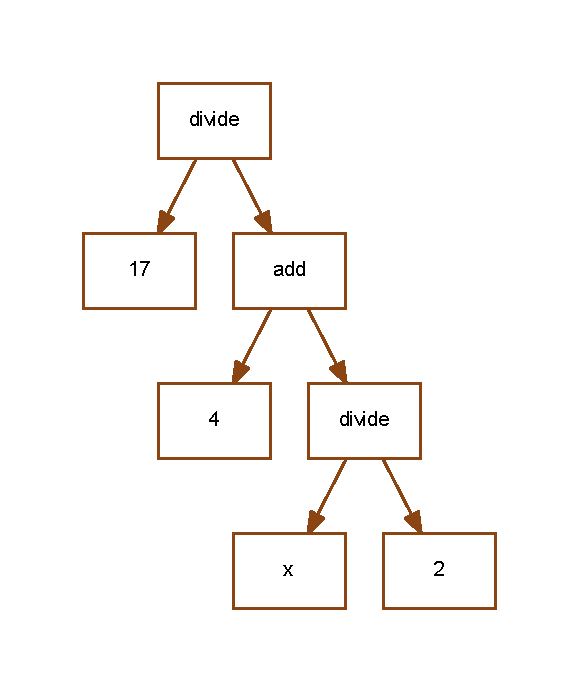
\includegraphics[scale=0.5]{pdf/semtree20.pdf}
\end{center}

\section{Terms}
We call the components of a prefix expression {\em terms}. Syntactically, we can define terms using an inductive (recursive) set of rules like this.
\begin{enumerate}
\item A symbol such \fbox{1}, \fbox{$\pi$} or \fbox{:=} is a term.
\item A symbol followed by a parenthesized comma-delimited list of terms is a term.
\end{enumerate}
Rule one defines terms made up of single symbols. Rule 2 is recursive,
and this allows us to construct terms of arbitrary depth by building
one upon another.

The {\em arity} of a term is the number of terms within its
parentheses. Terms from rule 1 have no parentheses: they are
arity-zero. Equivalently, the arity is the number of children a term
symbol has in its tree representation. Rule 1 terms have no children
and so are the leaves of a term tree.

Quite often, all instances of a symbol will have the same arity. For instance, addition is usually thought of as a binary (arity-two) operation, and an expression $3+4+5$ could be represented by the term \verb+add(add(3, 4),5)+. However, we could instead decide to have {\em variable} arity addition, in which case $4+4+5$ could be represented as \verb+add(3,4,5)+.


\subsection{Denoting term symbols}

We are very permissive about what constitutes a symbol. When we are thinking about theory, we allow the symbols to be any mathematical object. In this book, when we are thinking about computer based tools we shall allow a symbol to be {\em any} valid text string over the Unicode alphabet.

Now, great care is needed when reasoning about and writing down terms. Rule 2 above make comma and parentheses special: how would we go about writing a symbol that contained parentheses or command? We call these special characters {\em metacharacters} because they are used in the denotation of terms.
 
If we do want a parenthesis or a comma within a symbol, we usually write it with a
preceding back-slash (\verb+\( \) \,+ or sometimes back-quote
character. Of course, we have now added another meta-symbol, so if we
want a back-slash in a symbol name we have to write it as \verb+\\+.


\subsection{Typed terms}
Our definition of terms allows any term to be a subterm of any other term. Often we want to place constraints on our terms by limiting 
\section{Terms and their implementation in Java}
\label{TermsAndImplementation}
\newcommand{\str}{\mbox{\em Str}}
\newcommand{\nat}{\mbox{\em Nat}}
\newcommand{\obj}{\mbox{\em Obj}}

Assume that we have types \str (strings), \nat (natural numbers) and \obj (any data type). 

We can move from 
\begin{description}
\item [Pure text labels with embedded arity] $\str\ \mbox{label} \times \nat\ \mbox{arity} \times \mbox{term}^*$ 
\item [String map $\str\leftrightarrow\nat$]  $\nat\ \mbox{label} \times \nat\ \mbox{arity} \times \mbox{term}^*$
\item [Fixed arity map $\nat\leftrightarrow\nat$] $\nat\ \mbox{label} \times \nat\ \mbox{arity} \times \mbox{term}^* \lor \nat\ \mbox{label} \times \mbox{term}^*, \mbox{label} \in \mbox{arity map}$
\item [Types mapped to -1 in arity table, structure map $\nat\leftrightarrow\obj$] $\nat\ \mbox{label} \times \nat\ \mbox{data}$
\item [Small types bool, char, int and real mapped to negatives] $\nat\ \mbox{label} \times \mbox{data}$
\end{description}

Arrays should just be a vector of children



\label{rewriting:chapter}
\section{The Value system and plugins}
\chapter{Reduction semantics with eSOS}
\label{eSOS:chapter}
\chapter{Attribute action interpreters}
\label{attribute:chapter}
\chapter{Advice on language design}
\label{advice:chapter}
\appendix
\chapter{Music making with Java MIDI}
\label{music:chapter}
\chapter{Image processing operations}
\label{ip:chapter}
\chapter{3D modelling}
\label{3d:chapter}
\chapter{ART reference documentation}
\printnomenclature
\end{document}
